\documentclass{sduthesis}

% 引入用户配置文件
% ============================================================
% 山东大学论文模板 - 用户配置
% ============================================================
%
% 使用方法：只需修改下方的 \SDUSetup{...} 中的内容
%
% 支持的配置项：
%   module      - 模板模块，支持逗号分隔多模块组合：
%                undergraduate / master / blindreview
%                例：{master, blindreview}（硕博论文+盲审）
%                例：{undergraduate, blindreview}（本科+盲审）
%                盲审模块需与基础模块组合；单独使用自动回退本科
%                盲审模式：封面隐藏姓名/学号/导师，答辩委员会页整页跳过
%   title       - 论文标题
%   author      - 作者姓名
%   studentId   - 学号
%   school      - 学院
%   major       - 专业
%   supervisor  - 指导教师
%   year        - 年份（如 2025）
%   month       - 月份（如 6）
%
% master 模块额外配置项：
%   degree           - 学位类型（硕士/博士，默认硕士）
%   committeeChair   - 答辩委员会主席
%   committeeMembers - 答辩委员会委员（顿号分隔）
%   defenseDate      - 答辩日期
%   defensePlace     - 答辩地点
%
% 样式配置项（可选）：
%   lineSpread  - 行距倍数（默认 1.5）
%   pageLeft    - 左边距（默认 3cm）
%   pageRight   - 右边距（默认 3cm）
%   pageTop     - 上边距（默认 2.5cm）
%   pageBottom  - 下边距（默认 2.5cm）
%
% ============================================================

\SDUSetup{
  module     = {undergraduate},
  title      = {基于深度学习的图像识别研究},
  author     = {张三},
  studentId  = {2020123456},
  school     = {计算机科学与技术学院},
  major      = {计算机科学与技术},
  supervisor = {李四 教授},
  year       = {2025},
  month      = {6},
}


\begin{document}

% ==================== 前言 ====================
\frontmatter
\UseHook{sduthesis/frontmatter/begin}
\makecoverpage
% 中文摘要
\begin{cnabstract}

随着人工智能技术的飞速发展，图像识别作为计算机视觉领域的核心任务之一，在医疗诊断、自动驾驶、安防监控等领域发挥着越来越重要的作用。传统的图像识别方法依赖于人工设计的特征提取器，难以应对复杂多变的实际场景。近年来，深度学习技术的兴起为图像识别带来了新的突破，其中卷积神经网络（CNN）已成为该领域的主流方法。

本文针对图像识别中的关键技术问题展开研究，主要工作包括以下几个方面：首先，系统分析了卷积神经网络的基本原理和网络结构设计，探讨了残差网络（ResNet）、密集连接网络（DenseNet）等经典架构的优缺点；其次，针对现有模型参数量大、计算复杂度高的问题，提出了一种轻量级的改进网络结构，在保证识别精度的前提下显著降低了模型参数量和计算成本；最后，在CIFAR-10和ImageNet两个公开数据集上进行了大量实验验证，实验结果表明本文提出的方法相比基线模型具有更好的性能表现。

本文的研究工作为轻量化图像识别模型的设计提供了新的思路，对于推动深度学习在移动端和边缘设备上的应用具有重要的理论意义和实践价值。

\cnkeywords{图像识别；深度学习；卷积神经网络；残差网络；轻量级网络}
\end{cnabstract}

% 英文摘要
\begin{enabstract}

With the rapid development of artificial intelligence technology, image recognition, as one of the core tasks in the field of computer vision, plays an increasingly important role in medical diagnosis, autonomous driving, security surveillance and other fields. Traditional image recognition methods rely on manually designed feature extractors, which are difficult to cope with complex and changing real-world scenarios. In recent years, the rise of deep learning technology has brought new breakthroughs to image recognition, among which Convolutional Neural Networks (CNN) have become the mainstream method in this field.

This paper conducts research on key technical issues in image recognition. The main work includes the following aspects: Firstly, this paper systematically analyzes the basic principles of convolutional neural networks and network structure design, exploring the advantages and disadvantages of classic architectures such as Residual Network (ResNet) and Dense Network (DenseNet). Secondly, to address the problems of large parameter quantity and high computational complexity of existing models, a lightweight improved network structure is proposed, which significantly reduces model parameters and computational cost while ensuring recognition accuracy. Finally, extensive experimental verification is conducted on CIFAR-10 and ImageNet public datasets. Experimental results show that the proposed method has better performance compared with baseline models.

The research work in this paper provides new ideas for the design of lightweight image recognition models, and has important theoretical significance and practical value for promoting the application of deep learning on mobile terminals and edge devices.

\enkeywords{Image Recognition; Deep Learning; Convolutional Neural Network; Residual Network; Lightweight Network}
\end{enabstract}

\maketable

% ==================== 正文 ====================
\mainmatter
\UseHook{sduthesis/mainmatter/begin}
\chapter{绪论}

\section{研究背景与意义}

图像识别是计算机视觉领域的核心研究课题之一，其目标是通过计算机自动识别图像中的目标、场景或语义信息。随着数字图像获取技术的不断进步和互联网的快速发展，图像数据的规模呈指数级增长，如何高效准确地处理和理解这些海量图像数据已成为当前研究的热点问题。

在实际应用层面，图像识别技术已经渗透到社会生活的方方面面。在医疗领域，深度学习辅助诊断系统能够帮助医生更准确地识别医学影像中的病变区域，提高诊断效率和准确率\citing{esteva2017dermatologist}。在自动驾驶领域，车辆需要实时识别道路、行人、交通标志等多种目标，对识别算法的速度和精度都提出了极高要求\citing{grigorescu2020survey}。在安防监控领域，智能视频分析系统能够自动检测异常行为，为公共安全提供技术保障。

传统的图像识别方法主要基于手工设计的特征描述子，如尺度不变特征变换（SIFT）\citing{lowe2004distinctive}、方向梯度直方图（HOG）\citing{dalal2005histograms}等。这些方法在特定数据集上取得了较好的效果，但泛化能力有限，难以适应复杂多变的实际场景。2012年，Krizhevsky等人提出的AlexNet\citing{krizhevsky2012imagenet}在ImageNet图像分类挑战赛中取得了突破性成绩，标志着深度学习在图像识别领域的正式崛起。此后，VGGNet\citing{simonyan2014very}、GoogLeNet\citing{szegedy2015going}、ResNet\citing{he2016deep}等一系列更深更复杂的网络结构相继被提出，不断刷新着图像识别的性能指标。

尽管深度学习方法取得了显著成功，但现有的大部分高性能网络普遍存在参数量大、计算复杂度高的问题。以ResNet-152为例，其参数量超过6000万，需要超过20 GFLOPS的浮点运算才能完成单张图像的推理\citing{sandler2018mobilenetv2}。这使得这些模型难以部署到资源受限的移动端和边缘设备上。因此，研究如何在保证识别精度的前提下设计轻量化的网络模型，对于推动深度学习技术的广泛应用具有重要的理论意义和实用价值。

\section{国内外研究现状}

深度学习在图像识别领域的发展可以追溯到上世纪八九十年代的早期神经网络研究。LeCun等人提出的卷积神经网络LeNet-5\citing{lecun1998gradient}是最早的深度学习模型之一，被成功应用于手写数字识别。然而，由于当时计算资源的限制和训练数据的不足，深度学习的发展一度陷入瓶颈。

2006年，Hinton等人提出的深度置信网络（DBN）\citing{hinton2006fast}重新点燃了研究者对深度学习的热情。2012年是一个重要的转折点，AlexNet在ImageNet大规模视觉识别挑战赛（ILSVRC）中将Top-5错误率从之前的26.2\%降低到15.3\%，震惊了整个计算机视觉界。这一突破主要归功于以下几方面的进步：GPU并行计算能力的提升为大规模网络训练提供了硬件基础；ImageNet大规模标注数据集的建立解决了训练数据不足的问题；ReLU激活函数、Dropout正则化、GPU并行计算等技术的应用有效缓解了梯度消失和过拟合问题。

此后，深度卷积网络的研究进入了一个快速发展的时期。VGGNet\citing{simonyan2014very}通过使用更小的3×3卷积核堆叠更深的网络，证明了网络深度对模型性能的重要性。GoogLeNet\citing{szegedy2015going}提出的Inception模块通过多尺度卷积核并行设计，在大幅增加网络深度的同时有效控制了计算量。ResNet\citing{he2016deep}引入的残差连接机制解决了深层网络训练困难的问题，使得训练超过1000层的网络成为可能。DenseNet\citing{huang2017densely}通过密集连接进一步加强了特征复用，每层都直接接收所有前面层的特征作为输入。

在轻量化网络研究方面，MobileNetV1\citing{howard2017mobilenets}首次提出了深度可分离卷积（Depthwise Separable Convolution）的概念，将标准卷积分解为深度卷积和逐点卷积两步，大幅减少了计算量和参数量。MobileNetV2\citing{sandler2018mobilenetv2}在此基础上引入了线性瓶颈和倒残差结构，进一步提升了性能。ShuffleNet\citing{zhang2018shufflenet}则通过通道混洗操作加强了分组卷积模块的信息流动。EfficientNet\citing{tan2019efficientnet}系统地研究了网络深度、宽度和分辨率的平衡关系，通过复合缩放策略实现了性能和效率的最优权衡。

\section{主要研究内容}

本文围绕图像识别中的轻量化网络设计问题展开研究，主要研究内容如下：

\begin{enumerate}
    \item \textbf{系统分析深度学习图像识别技术}\\
        对卷积神经网络的基本原理进行全面梳理，深入分析激活函数、池化操作、归一化方法等核心组件的作用机制。比较研究ResNet、DenseNet等经典网络架构的设计思想和性能特点，为后续改进工作奠定理论基础。

    \item \textbf{提出轻量化改进网络结构}\\
        针对现有轻量级网络在特征提取能力上的不足，设计一种改进的轻量化网络模块。通过改进残差连接方式、优化通道注意力机制，在保持模型轻量化的同时增强特征表达能力。

    \item \textbf{搭建实验平台并进行验证}\\
        构建完整的实验系统，在CIFAR-10和ImageNet等标准数据集上进行大量对比实验。设计多组消融实验分析各改进模块的贡献，并通过可视化技术直观展示模型的学习效果。

    \item \textbf{开发图像识别原型系统}\\
        基于所提出的轻量化网络模型，开发一个完整的图像识别原型系统。系统支持模型量化压缩和移动端部署，能够在实际应用场景中验证算法的有效性。
\end{enumerate}

\section{论文结构安排}

本论文共分为六章，各章内容安排如下：

\textbf{第一章 绪论}——阐述课题的研究背景与意义，分析国内外研究现状，明确本文的主要研究内容和论文结构安排。

\textbf{第二章 相关技术与理论基础}——介绍卷积神经网络的基本原理和经典架构，讨论轻量化网络的设计策略，为后续研究提供理论支撑。

\textbf{第三章 系统设计与实现}——详细描述本文提出的轻量化改进网络结构，包括整体架构设计、核心模块实现和关键技术细节。

\textbf{第四章 实验与分析}——搭建实验平台，设计对比实验和消融实验，对所提方法的性能进行全面评估和分析。

\textbf{第五章 总结与展望}——总结本文的研究工作和主要贡献，指出研究的局限性，并对未来研究方向进行展望。

\chapter{相关技术与理论基础}

\section{卷积神经网络基本原理}

卷积神经网络是一类专门用于处理具有网格结构数据（如图像）的深度神经网络。与传统全连接神经网络相比，卷积神经网络通过局部连接和权重共享机制大幅减少了参数量，更适合处理高维图像数据。

\subsection{卷积层}

卷积层是卷积神经网络的核心组件，其主要功能是自动学习输入图像的特征表示。如图\ref{fig:convolution}所示，卷积操作通过一个可学习的卷积核（也称为滤波器）在输入图像上滑动，对局部区域进行加权求和运算。

\begin{figure}[htbp]
    \centering
    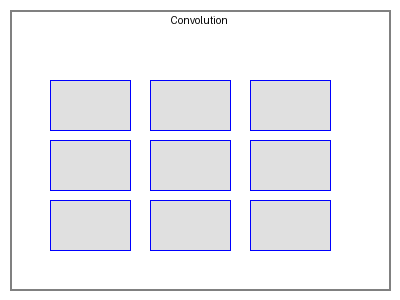
\includegraphics[width=0.7\textwidth]{assets/figures/convolution.png}
    \caption{卷积操作示意图}
    \label{fig:convolution}
\end{figure}

卷积运算的数学表达式如式\eqref{eq:conv}所示：

\begin{equation}
    y_{i,j} = \sum_{m}\sum_{n} w_{m,n} \cdot x_{i+m,j+n} + b
    \label{eq:conv}
\end{equation}

其中，$w_{m,n}$表示卷积核的权重，$b$为偏置项，$x_{i,j}$和$y_{i,j}$分别为输入和输出特征图的像素值。

卷积操作具有以下三个重要特性：

\begin{itemize}
    \item \textbf{局部连接}：每个神经元只与输入数据的局部区域相连，局部区域的大小称为感受野。这使得网络能够提取局部特征，同时减少参数量。
    \item \textbf{权重共享}：同一个卷积核在滑动过程中使用相同的权重参数。这大大减少了需要学习的参数数量，提高了网络的泛化能力。
    \item \textbf{平移不变性}：由于权重共享机制，网络对输入目标的平移、旋转等变换具有一定的不变性。
\end{itemize}

\subsection{激活函数}

激活函数为神经网络引入非线性变换，使其能够拟合复杂的非线性函数。常用的激活函数包括ReLU、Sigmoid和Tanh等。ReLU函数的表达式如式\eqref{eq:relu}所示：

\begin{equation}
    f(x) = \max(0, x)
    \label{eq:relu}
\end{equation}

ReLU函数计算简单，收敛速度快，是目前应用最广泛的激活函数。然而，ReLU神经元在训练过程中可能出现"死亡"问题，即当输入长期为负时，梯度始终为0，神经元将不再更新。

\subsection{池化层}

池化层（Pooling Layer）通过对特征图进行下采样来减少特征图的尺寸，同时保留重要的特征信息。常用的池化操作包括最大池化（Max Pooling）和平均池化（Average Pooling）。

\begin{figure}[htbp]
    \centering
    \subfloat[最大池化]{
        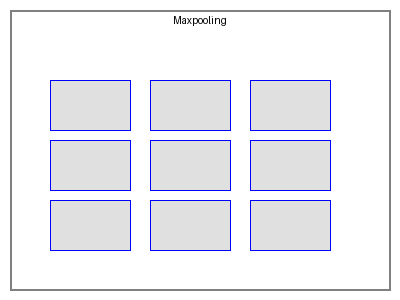
\includegraphics[width=0.45\textwidth]{assets/figures/maxpooling.png}
    }
    \subfloat[平均池化]{
        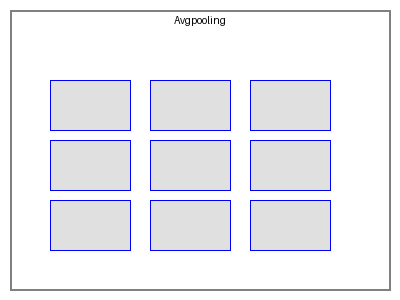
\includegraphics[width=0.45\textwidth]{assets/figures/avgpooling.png}
    }
    \caption{池化操作示意图}
    \label{fig:pooling}
\end{figure}

图\ref{fig:pooling}展示了这两种池化操作的计算过程。最大池化选择局部区域中的最大值，能够保留纹理特征；平均池化计算局部区域的平均值，使特征更加平滑。

\section{经典网络架构}

\subsection{残差网络ResNet}

随着网络层数的增加，研究者发现简单的堆叠卷积层会导致网络性能下降，这种现象称为网络退化。He等人提出的ResNet\citing{he2016deep}通过引入残差连接（Skip Connection）巧妙地解决了这一问题。

残差块的基本结构如图\ref{fig:resblock}所示。假设原始映射为$\mathcal{H}(x)$，残差映射为$\mathcal{F}(x) = \mathcal{H}(x) - x$。残差块学习的目标从直接学习$\mathcal{H}(x)$转变为学习残差$\mathcal{F}(x)$。当残差为0时，该结构相当于恒等映射，网络性能至少不会下降；当残差不为0时，网络能够学习到新的特征。

\begin{figure}[htbp]
    \centering
    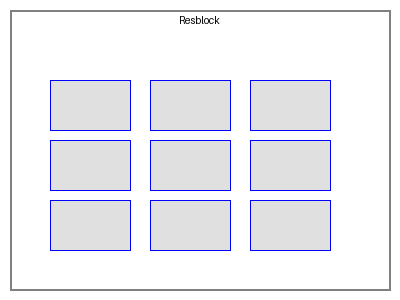
\includegraphics[width=0.5\textwidth]{assets/figures/resblock.png}
    \caption{残差块结构}
    \label{fig:resblock}
\end{figure}

残差连接的数学表达式如式\eqref{eq:residual}所示：

\begin{equation}
    y = \mathcal{F}(x, \{W_i\}) + x
    \label{eq:residual}
\end{equation}

ResNet通过堆叠多个残差块，成功训练了超过1000层的深度网络，在ImageNet数据集上将Top-5错误率降低到3.57\%。

\subsection{密集连接网络DenseNet}

Huang等人提出的DenseNet\citing{huang2017densely}采用了更为激进的连接方式——密集连接。在DenseNet中，每一层都接收所有前面层的特征图作为输入，同时将自己的特征图传递给所有后续层。

假设网络共有$L$层，密集连接可以表示为：

\begin{equation}
    x_l = H_l([x_0, x_1, \ldots, x_{l-1}])
    \label{eq:dense}
\end{equation}

其中$[x_0, x_1, \ldots, x_{l-1}]$表示前面所有层特征图的拼接，$H_l(\cdot)$表示第$l$层的非线性变换。

DenseNet的这种密集连接方式具有以下优点：加强了特征复用，减少了参数量；缓解了梯度消失问题；每层都可以直接访问损失函数的梯度，实现了隐式的深度监督。

\section{轻量化网络设计策略}

\subsection{深度可分离卷积}

深度可分离卷积（Depthwise Separable Convolution）是轻量化网络设计的核心技术，被广泛应用于MobileNet系列网络。其基本思想是将标准卷积分解为两个独立的步骤：深度卷积和逐点卷积。

标准卷积的计算量为：

\begin{equation}
    D_K \times D_K \times M \times N \times D_F \times D_F
\end{equation}

深度可分离卷积的计算量为：

\begin{equation}
    D_K \times D_K \times M \times D_F \times D_F + M \times N \times D_F \times D_F
\end{equation}

两者的计算量之比为：

\begin{equation}
    \frac{1}{N} + \frac{1}{D_K^2}
    \label{eq:dsc_ratio}
\end{equation}

当卷积核大小为$3 \times 3$时，深度可分离卷积的计算量仅为标准卷积的$\frac{1}{8}$到$\frac{1}{9}$。

\subsection{通道注意力机制}

通道注意力机制通过自适应地调整不同通道的权重，使网络能够聚焦于更重要的特征通道。SE-Net\citing{hu2018squeezeandexcitation}提出的Squeeze-and-Excitation（SE）模块是通道注意力的经典实现。

SE模块包含两个关键操作：Squeeze（压缩）和Excitation（激发）。Squeeze操作通过全局平均池化将每个通道压缩为一个标量；Excitation操作通过两个全连接层学习通道间的依赖关系。SE模块的输出如式\eqref{eq:se}所示：

\begin{equation}
    s = \sigma(W_2 \delta(W_1 y_{avg}))
    \label{eq:se}
\end{equation}

其中$\delta$为ReLU激活函数，$\sigma$为Sigmoid激活函数，$W_1$和$W_2$为两个全连接层的权重矩阵。

\section{本章小结}

本章系统介绍了卷积神经网络的基本原理，包括卷积层、激活函数和池化层等核心组件的工作机制。重点分析了ResNet和DenseNet两种经典网络架构的设计思想和创新点。最后，讨论了轻量化网络的主要设计策略，为后续章节的改进工作奠定了理论基础。

\chapter{图表示例}

\section{插图}

图片通常在 \texttt{figure} 环境中使用 \texttt{\textbackslash includegraphics} 插入，如图~\ref{fig:example} 的源代码。
建议矢量图片使用 PDF 格式，比如数据可视化的绘图；
照片应使用 JPG 格式；
其他的栅格图应使用无损的 PNG 格式。
注意，LaTeX 不支持 TIFF 格式；EPS 格式已经过时。

\begin{figure}[htbp]
  \centering
  
\includegraphics[width=0.5\linewidth]{logos/sdu_logo_1.pdf}
  \caption{示例图片标题}
  \label{fig:example}
\end{figure}

若图或表中有附注，采用英文小写字母顺序编号，附注写在图或表的下方。
国外的期刊习惯将图表的标题和说明文字写成一段，需要改写为标题只含图表的名称，其他说明文字以注释方式写在图表下方，或者写在正文中。

如果一个图由两个或两个以上分图组成时，各分图分别以 (a)、(b)、(c)...... 作为图序，并须有分图题。
推荐使用 \texttt{subfig} 宏包来处理， 比如图~\ref{fig:subfig-a} 和图~\ref{fig:subfig-b}。

\begin{figure}[htbp]
  \centering
  \subfloat[分图 A\label{fig:subfig-a}]{
    
\includegraphics[width=0.35\linewidth]{logos/sdu_logo_1.pdf}
  }
  \hspace{0.05\linewidth}
  \subfloat[分图 B\label{fig:subfig-b}]{
    
\includegraphics[width=0.35\linewidth]{logos/sdu_logo_2.pdf}
  }
  \caption{多个分图的示例}
  \label{fig:multi-image}
\end{figure}



\section{表格}

表应具有自明性。表中参数应标明量和单位的符号。
为使表格简洁易读，均采用三线表（例如表~\ref{tab:three-line}）。
必要时可加辅助线，三线表无法清晰表达时可采用其他格式。

表序与表题置于表的上方。表单元格中的文字一般应居中书写（上下居中，左右居中），
不宜左右居中书写的，可采取两端对齐的方式书写。

\begin{table}[htbp]
  \centering
  \caption{三线表示例}
  \begin{tabular}{cc}
    \toprule
    文件名          & 描述                         \\
    \midrule
    sduthesis.cls   & 模板文件                     \\
    main.tex        & 主文件                       \\
    sdusetup.tex    & 用户配置文件                 \\
    \bottomrule
  \end{tabular}
  \label{tab:three-line}
\end{table}

若表中有附注，采用英文小写字母顺序编号，附注写在表的下方。

如某个表需要转页接排，可以"续表"的形式另页打印，格式同前，只需在每页表序前加"续"字即可。
续表均应重复表头。



\section{算法}

算法环境可以使用 \texttt{algorithm2e} 宏包。

\begin{algorithm}[htbp]
  \caption{计算 $y = x^n$}
  \label{alg:power}
  \KwIn{$n \geq 0$}
  \KwOut{$y = x^n$}
  
  $y \leftarrow 1$\;
  $X \leftarrow x$\;
  $N \leftarrow n$\;
  
  \While{$N \neq 0$}{
    \eIf{$N$ 是偶数}{
      $X \leftarrow X \times X$\;
      $N \leftarrow N / 2$\;
    }{
      $y \leftarrow y \times X$\;
      $N \leftarrow N - 1$\;
    }
  }
  \Return{$y$}\;
\end{algorithm}

\chapter{数学符号和公式}

\section{数学符号}

中文论文的数学符号默认遵循 GB/T 3102.11—1993《物理科学和技术中使用的数学符号》
\footnote{原 GB 3102.11—1993，自 2017 年 3 月 23 日起，该标准转为推荐性标准。}。
该标准参照采纳 ISO 31-11:1992 \footnote{目前已更新为 ISO 80000-2:2019。}，
但是与 \TeX{} 默认的美国数学学会（AMS）的符号习惯有所区别。
具体地来说主要有以下差异：
\begin{enumerate}
  \item 大写希腊字母默认为斜体，如
    \begin{equation*}
      \Gamma \Delta \Theta \Lambda \Xi \Pi \Sigma \Upsilon \Phi \Psi \Omega.
    \end{equation*}
  \item 小于等于号和大于等于号使用倾斜的字形 $\le$、$\ge$。
  \item 积分号使用正体，比如 $\int$、$\oint$。
  \item 偏微分符号 $\partial$ 使用正体。
  \item 省略号按照中文的习惯固定居中，比如
    \begin{equation*}
      1, 2, \dots, n \quad 1 + 2 + \dots + n.
    \end{equation*}
  \item 实部 $\Re$ 和虚部 $\Im$ 的字体使用罗马体。
\end{enumerate}

以上数学符号样式的差异可以在模板中统一设置。
另外国标还有一些与 AMS 不同的符号使用习惯，需要用户在写作时进行处理：
\begin{enumerate}
  \item 数学常数和特殊函数名用正体，如
    \begin{equation*}
      \pi = 3.14\dots; \quad
      i^2 = -1; \quad
      e = \lim_{n \to \infty} \left( 1 + \frac{1}{n} \right)^n.
    \end{equation*}
  \item 微分号使用正体，比如 $\mathrm{d} y / \mathrm{d} x$。
  \item 向量、矩阵和张量用粗斜体，如 $\mathbf{x}$、$\mathbf{\Sigma}$。
  \item 自然对数用 $\ln x$ 不用 $\log x$。
\end{enumerate}



\section{数学公式}

数学公式可以使用 \texttt{equation} 和 \texttt{equation*} 环境。
注意数学公式的引用应前后带括号，通常使用 \texttt{\textbackslash eqref} 命令，比如式~\eqref{eq:example}。
\begin{equation}
  \frac{1}{2 \pi i} \int_\gamma f = \sum_{k=1}^m n(\gamma; a_k) \mathscr{R}(f; a_k).
  \label{eq:example}
\end{equation}

多行公式尽可能在"="处对齐，推荐使用 \texttt{align} 环境。
\begin{align}
  a & = b + c + d + e \\
    & = f + g
\end{align}



\section{数学定理}

定理环境的格式可以使用 \texttt{amsthm} 宏包配置。
模板已经配置了 \texttt{theorem}、\texttt{proof} 等环境。

\begin{theorem}[Lindeberg--Lévy 中心极限定理]
  设随机变量 $X_1, X_2, \dots, X_n$ 独立同分布， 且具有期望 $\mu$ 和有限的方差 $\sigma^2 \ne 0$，
  记 $\bar{X}_n = \frac{1}{n} \sum_{i=1}^n X_i$，则
  \begin{equation}
    \lim_{n \to \infty} P \left(\frac{\sqrt{n} \left( \bar{X}_n - \mu \right)}{\sigma} \le z \right) = \Phi(z),
  \end{equation}
  其中 $\Phi(z)$ 是标准正态分布的分布函数。
\end{theorem}
\begin{proof}
  显然成立。
\end{proof}

\chapter{引用文献的标注}

模板使用 BibLaTeX 配合 GB/T 7714-2015 样式处理参考文献。


\section{文献引用}

在顺序编码制下，默认的 \texttt{\textbackslash cite} 命令会将序号置于方括号中。
统一处引用的连续序号会自动用短横线连接。

\noindent
\begin{tabular}{l@{\quad 示例：\quad}l}
  \verb|\cite{key}|           & 引用单篇文献               \\
  \verb|\cite{key1,key2}|     & 引用多篇文献               \\
  \verb|\cite[42]{key}|       & 引用文献的特定页码         \\
\end{tabular}



\section{参考文献列表}

参考文献列表会自动生成在论文末尾。
参考文献的每条都要在正文中标注引用。

文献数据库文件默认为 \texttt{assets/data/references.bib}，
可以在 \texttt{sdusetup.tex} 中修改路径。

参考文献的格式遵循 GB/T 7714-2015《信息与文献 参考文献著录规则》国家标准。



\section{文献管理建议}

\begin{enumerate}
  \item 使用文献管理软件（如 Zotero、Mendeley）管理参考文献
  \item 及时导出 BibTeX 格式的文献数据库
  \item 检查文献信息的完整性和准确性
  \item 确保所有引用的文献都在数据库中
  \item 删除未引用的文献条目
\end{enumerate}


% ==================== 附录 ====================
% 附录必须在 \backmatter 之前：\appendix 依赖 \@mainmattertrue 才能为
% 章节生成“附录A/B/C”编号（\backmatter 会关闭章节编号）。
\begin{myappendix}
% 附录
% 如果不需要附录，可以删除此文件或注释掉 main.tex 中的引用

\chapter{攻读学位期间发表的学术论文}

\begin{enumerate}
    \item 张三, 李四. 基于深度学习的图像识别算法研究[J]. 计算机科学与探索, 2024, 18(5): 123-135.
    \item 张三, 王五, 李四. 一种轻量化卷积神经网络的设计与实现[C]// 第33届中国机器学习会议论文集. 2024: 456-467.
\end{enumerate}

\chapter{补充实验数据}

\section{网络各层详细参数统计}

表\ref{tab:layer_params}列出了本文提出的网络模型各层的详细参数分布情况。

\begin{table}[htbp]
    \centering
    \caption{网络各层参数统计}
    \begin{tabular}{cccc}
        \toprule
        \textbf{层类型} & \textbf{数量} & \textbf{参数量(M)} & \textbf{占比(\%)} \\
        \midrule
        $1\times1$ 卷积 & 12 & 0.82 & 25.6 \\
        $3\times3$ 深度卷积 & 15 & 0.34 & 10.6 \\
        $1\times1$ 点卷积 & 15 & 1.65 & 51.6 \\
        归一化层 & 30 & 0.02 & 0.6 \\
        全连接层 & 1 & 0.37 & 11.6 \\
        \bottomrule
    \end{tabular}
    \label{tab:layer_params}
\end{table}

\section{超参数敏感性分析}

图\ref{fig:hyperparam}展示了学习率和批次大小对模型性能的影响曲线。从实验结果可以看出，学习率为0.001时模型性能最优；批次大小过小会导致梯度估计不稳定，批次大小过大会降低模型的泛化能力。

\begin{figure}[htbp]
    \centering
    \subfloat[学习率]{
        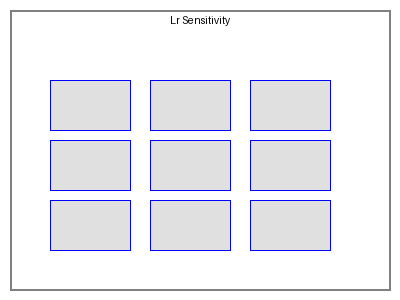
\includegraphics[width=0.45\textwidth]{assets/figures/lr_sensitivity.png}
    }
    \subfloat[批次大小]{
        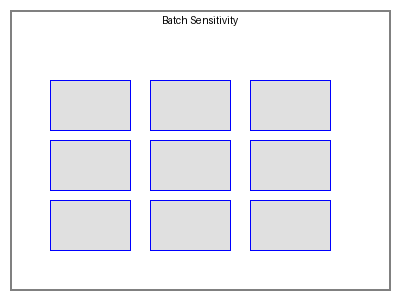
\includegraphics[width=0.45\textwidth]{assets/figures/batch_sensitivity.png}
    }
    \caption{超参数敏感性分析}
    \label{fig:hyperparam}
\end{figure}

\chapter{代码实现补充说明}

\section{模型定义核心代码}

以下是改进轻量化模块的核心实现代码：

\begin{verbatim}
// Enhanced Lite Block 核心实现
class EnhancedLiteBlock(nn.Module):
    def __init__(self, in_channels, out_channels, stride=1):
        super().__init__()
        # 深度可分离卷积
        self.dw_conv = nn.Conv2d(in_channels, in_channels, 3, 
                                 stride=stride, padding=1, 
                                 groups=in_channels)
        # 通道注意力
        self.ca = ChannelAttention(in_channels)
        # 逐点卷积
        self.pw_conv = nn.Conv2d(in_channels, out_channels, 1)
        # 增强残差连接
        if stride != 1 or in_channels != out_channels:
            self.shortcut = nn.Conv2d(in_channels, out_channels, 1, stride)
        else:
            self.shortcut = nn.Identity()
    
    def forward(self, x):
        identity = self.shortcut(x)
        out = self.dw_conv(x)
        out = self.ca(out)
        out = self.pw_conv(out)
        return out + identity
\end{verbatim}

\section{实验环境详细配置}

\begin{itemize}
    \item \textbf{操作系统}：Ubuntu 20.04 LTS
    \item \textbf{CPU}：Intel Xeon Gold 6248R @ 3.00GHz
    \item \textbf{GPU}：NVIDIA Tesla V100 32GB
    \item \textbf{深度学习框架}：PyTorch 2.0.1
    \item \textbf{Python版本}：3.10.12
    \item \textbf{CUDA版本}：11.8
\end{itemize}

\end{myappendix}

% ==================== 后记 ====================
\backmatter
\UseHook{sduthesis/backmatter/begin}
\printbib
\begin{myacknowledgement}
\begin{myacknowledgement}

    时光荏苒，四年的本科学习生活即将画上圆满的句号。在论文完成之际，我怀着崇敬和感激的心情，向在我大学四年学习和生活中给予我帮助和支持的老师、同学、家人致以最诚挚的谢意。

    首先，我要衷心感谢我的指导教师李教授。从选题确定、文献综述到实验设计和论文撰写，李老师都给予了我悉心的指导和耐心的帮助。李老师严谨求实的治学态度、渊博的学术知识和孜孜不倦的敬业精神深深影响了我，这将是我一生受用的宝贵财富。在此，向李老师表示崇高的敬意和衷心的感谢！

    其次，感谢计算机科学与技术学院的各位老师。感谢你们在专业课程教学中的精心讲授，为我奠定了扎实的理论基础。感谢学院提供的良好学习环境和实验条件，使我的研究工作能够顺利开展。

    感谢实验室的同学们，特别感谢王同学和张同学在实验过程中的帮助与讨论。每周的组会交流让我受益匪浅，你们的建议和鼓励是我不断前进的动力。感谢你们在繁忙的研究工作中抽出时间与我探讨问题、分享经验。

    感谢我的家人。感谢父母多年来的养育之恩和默默付出，是你们的支持和鼓励让我能够专注于学业，顺利完成大学四年学习。你们无条件的爱和信任是我最坚强的后盾，激励着我不断追求进步。

    感谢山东大学图书馆提供的丰富学术资源，感谢所有参考文献的作者们，你们的研究工作为本论文提供了重要的理论基础和参考依据。

    最后，向在百忙之中抽出时间评审本论文的各位专家和学者表示诚挚的谢意！

    \vspace{2cm}
    \begin{flushright}
        作者签名：\underline{\hspace{3cm}}\\
        \vspace{0.5cm}
        二〇二四年六月于山东大学
    \end{flushright}

\end{myacknowledgement}

\end{myacknowledgement}

\end{document}
